\section{Approach}\label{sec:approach}

\subsection{Overview}\label{subsec:overview}

Although this project is framed as a ``pipeline,'' in practice, the development was semi-structured,
exploratory, and highly interactive.
The overall goal was to translate technical research papers into short comics with minimal manual effort,
guided by large language models and image generation systems.
Rather than designing a rigid system, the process unfolded through iterative experimentation,
often driven by intuition and model feedback.
The workflow blended prompt design, model iteration, and lightweight scripting to orchestrate a reproducible but flexible method.

\subsection{Scene Planning and Narrative Structuring}\label{subsec:scene-planning-and-narrative-structuring}

The first stage involved asking the LLM to interpret a full research paper and propose
a scene structure appropriate for comic storytelling.
Instead of using a fixed template, the number and content of scenes were dynamically adapted based on the paper's complexity and focus.
In many cases, the LLM was able to identify key concepts (e.g., problem, method, insight, results) and organize them
into sequential scenes with minimal user correction.
This narrative framing included not only technical explanations but also character-driven setups designed to make abstract ideas more engaging.

\subsection{Dialogue and Panel Generation}\label{subsec:dialogue-and-panel-generation}

Each scene was described using a single prompt that asked the LLM to generate four panels, including setting,
character actions, and dialogue.
The generated dialogue aimed to balance technical accuracy with accessibility.
This stage often involved multi-turn conversations, as refining the scene with the model
(e.g., confirming character tone, simplifying explanations) consistently produced more coherent output than one-shot prompting.

\subsection{Image Generation and Prompt Strategy}\label{subsec:image-generation-and-prompt-strategy}

Initially, diffusion-based image models were used to render comic panels.
Because these models struggled with in-image text rendering, dialogue was overlaid using HTML\@.
Prompts were structured to include characters, actions, and visual tone while avoiding excessive detail.
One of the earliest challenges was character inconsistency across panels.
After testing multiple strategies, the most effective method involved using character names as stable anchor points in the prompt.

Following the release of OpenAI's updated image generation tools (GPT-4o, March 25, 2025),
two new features reshaped the project: significantly improved in-image text rendering and support for character consistency.
Early tests showed strong improvements in visual quality, with legible dialogue and recognizable characters.
However, when prompting the model to ``reuse the same characters'' directly, results were mixed.
I discovered that generating a reference image first --- one showing all characters without background
or interaction --- greatly improved consistency in subsequent scene generation.
Because the new model supports multiple panels per image,
I also shifted from generating four separate images to producing a single 2x2 layout in one shot.
While this sacrifices some detail compared to single-panel generation,
the gains in coherence and workflow efficiency make it a worthwhile tradeoff.


To further evaluate this shift, I generated two sets of reference images.
Each set includes a group portrait of the three main characters,
and two additional images showing character pairs (C1 and C2, C2 and C3) interacting.
Figure~\ref{fig:char-new-row} shows the results using the older diffusion-based model,
while Figure~\ref{fig:char-old-row} shows  the equivalent outputs from the new autoregressive model.
These comparisons highlight the improvements in character retention and scene-level coherence achieved with the newer approach.

\begin{figure*}[ht]
    \centering

    \begin{subfigure}[t]{0.48\linewidth}
        \centering
        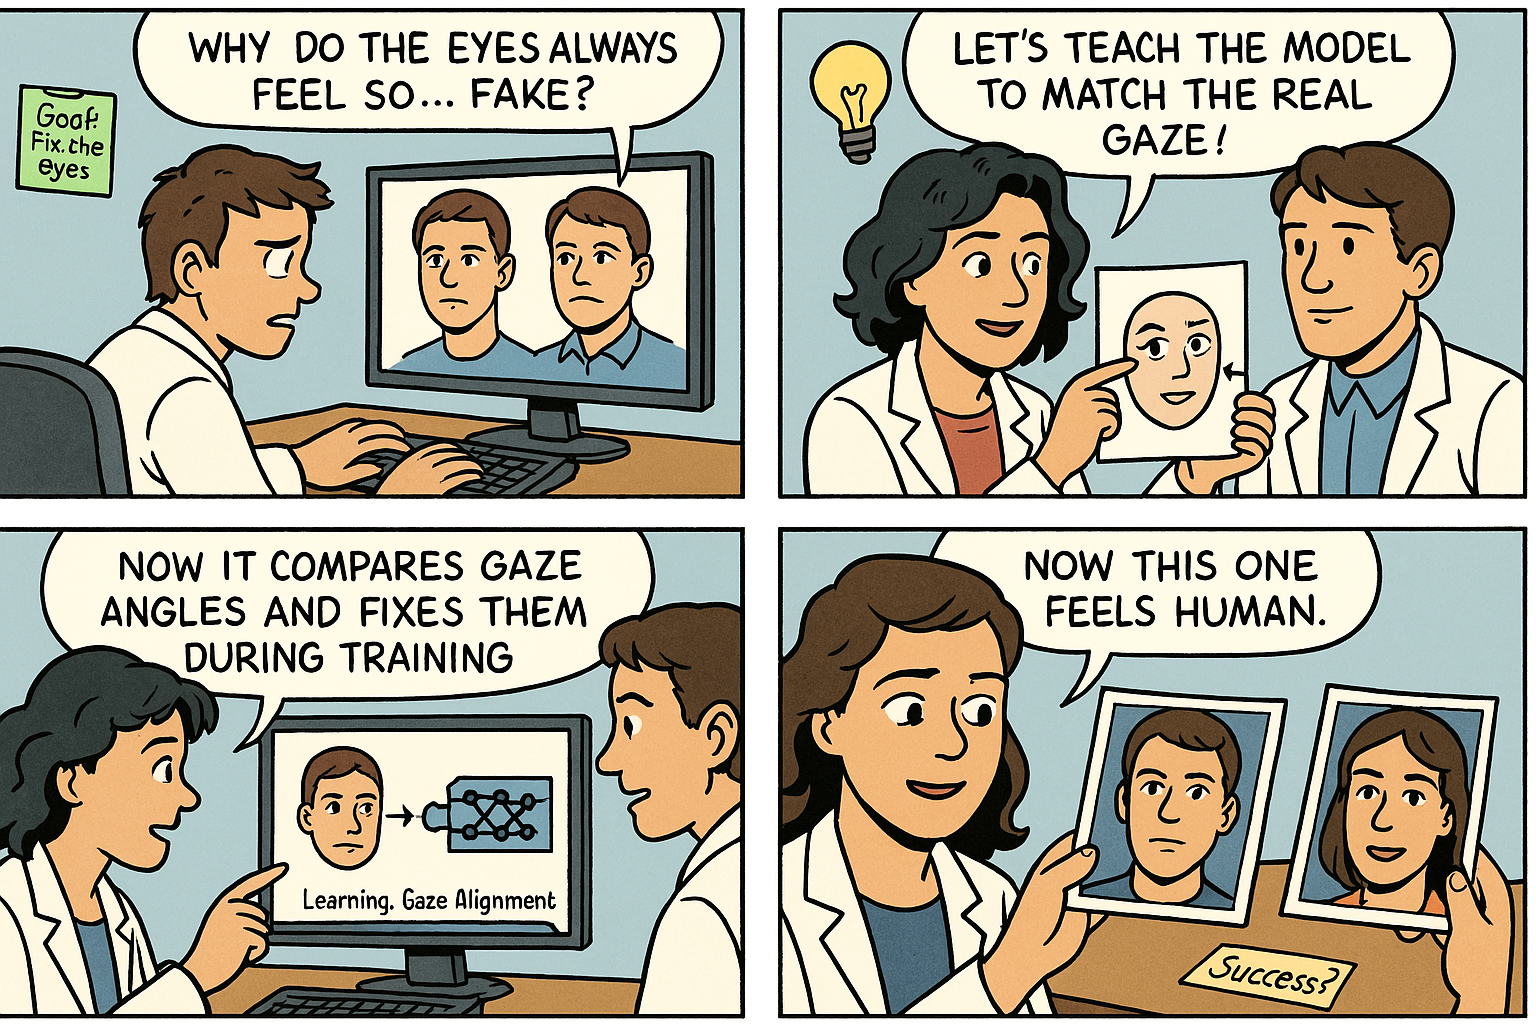
\includegraphics[height=0.7\linewidth]{resources/less_detailed.png}
        \caption{Simplified prompt}
        \label{fig:prompt-simple}
    \end{subfigure}
    \hspace{0.02\linewidth}
    \begin{subfigure}[t]{0.48\linewidth}
        \centering
        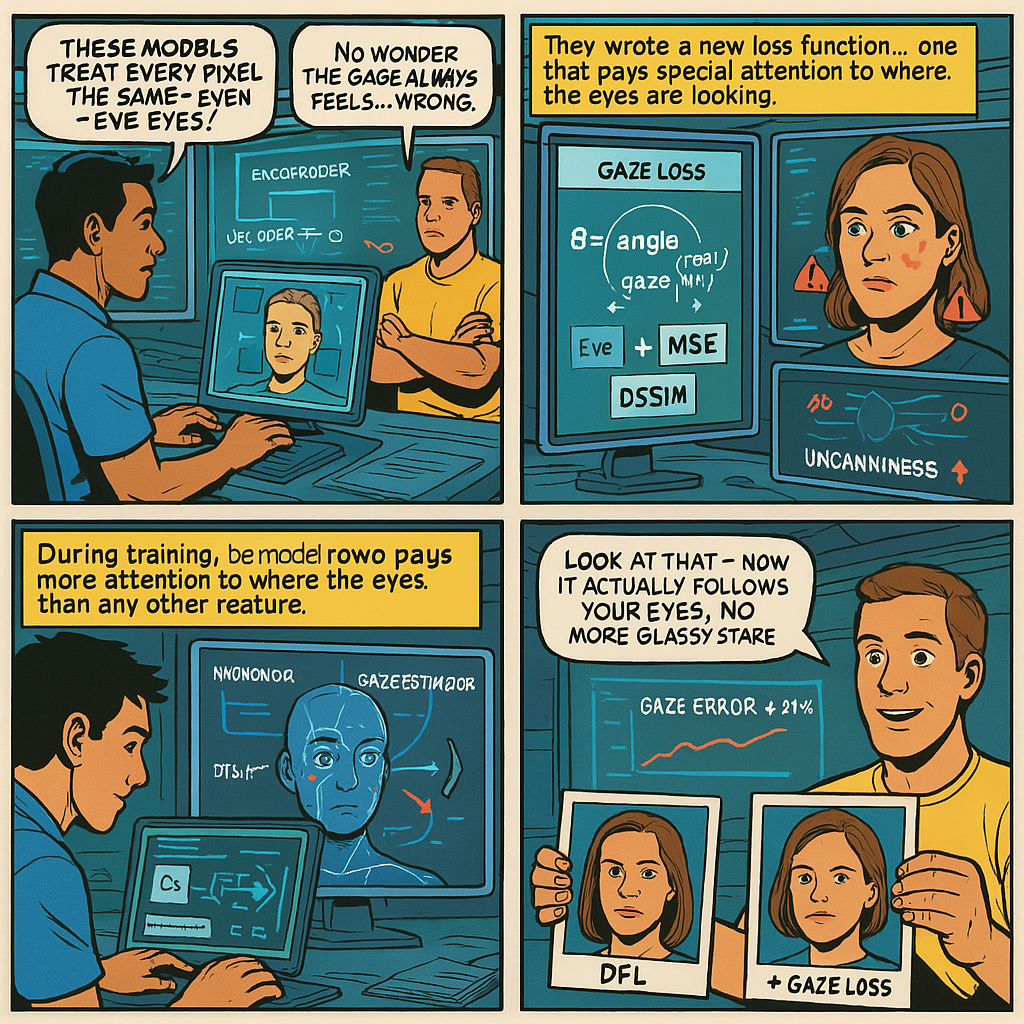
\includegraphics[height=0.7\linewidth]{resources/too_much_details.png}
        \caption{Overly detailed prompt}
        \label{fig:prompt-detailed}
    \end{subfigure}

    \caption{Comparison between simplified and overly detailed prompts for the same scene. The simplified prompt results in more coherent and complete image generation, while the overly detailed version caused truncation and hallucination.}
    \label{fig:prompt-detail-comparison}
\end{figure*}


Additionally, I tested the effect of prompt complexity on image quality.
Two versions of the same scene from~\cite{wilson2024towards} were created:
one from a highly detailed prompt and another from a simplified version.
The outputs are shown in Figure~\ref{fig:prompt-detail-comparison};
detailed prompt contents can be found in Appendix~\ref{sec:prompt-details-for-scene-comparison}.

\subsection{Data Structuring and Rendering}\label{subsec:data-structuring-and-rendering}

To streamline generation and output formatting, the dialogue and image metadata were converted into
JSON format with the help of the LLM\@.
A Python script sorted and organized image files by name and aligned them with their corresponding text.
The final output was rendered using a simple HTML layout that supports clean text overlays and scalable presentation.

\subsection{Semi-Automation and Human Feedback Loops}\label{subsec:semi-automation-and-human-feedback-loops}

Throughout the pipeline, the LLM served not just as a generator but as a collaborator.
I used it to reformat dialogue, clarify ambiguous outputs, and self-evaluate the coherence of generated scenes.
Even simple interactions --- such as asking the model to confirm a response before continuing—improved downstream image quality.
This reflects a broader insight: human-AI collaboration is most effective when framed as an ongoing dialogue, not a single request.
